\documentclass[11pt]{wbzine}
%packages
\usepackage{lipsum}
\usepackage[utf8]{inputenc}
\usepackage[T1]{fontenc}
\usepackage[ngerman]{babel}
\usepackage{coelacanth}
\usepackage{pdfpages}

\begin{document}

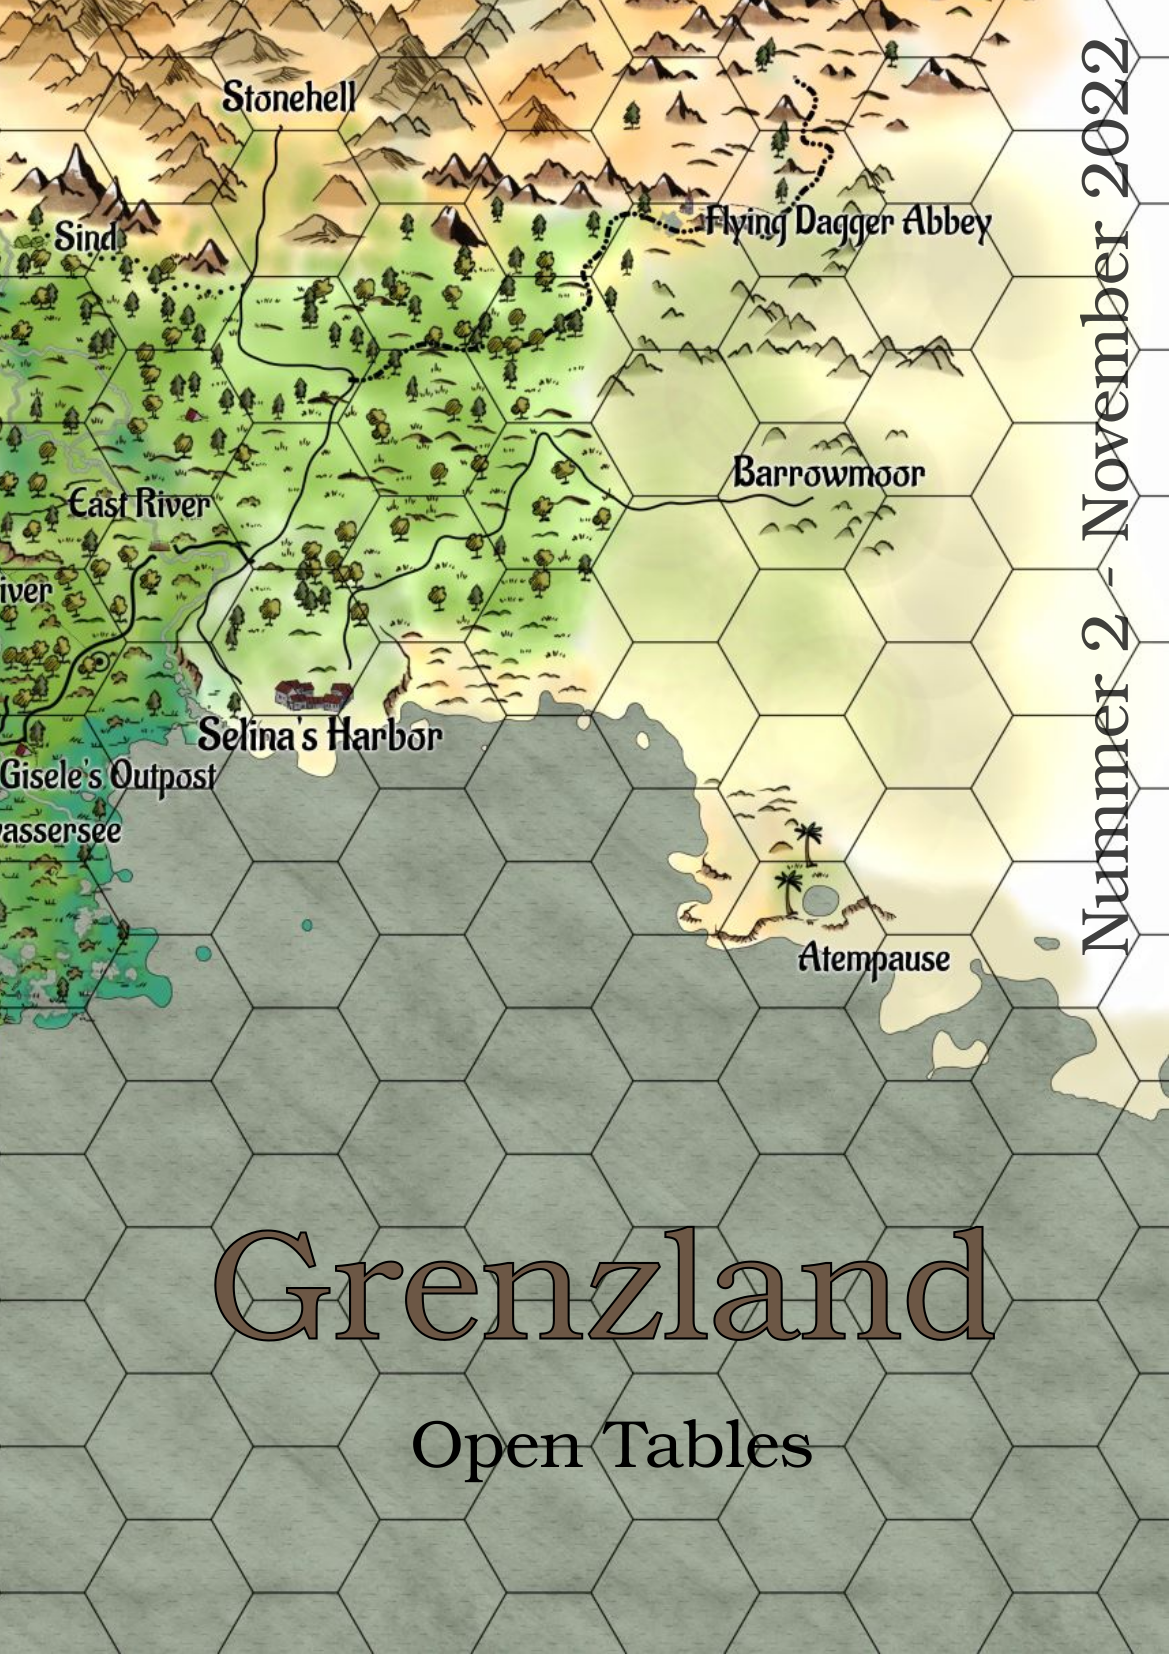
\includepdf{Frontcover.pdf}

{\bfseries\fontsize{70}{55}
 \selectfont Grenzland \par}%
 \hrulefill
 Nummer 2, November 2022

\tableofcontents

\begin{multicols}{2}

\section{Vorwärts!}

Hier das Vorwort. Aber erst wenn alles andere fertig ist ...

\section{Was wird gespielt?}

Hier finden sich Infos und Beschreibungen zu den Spielen die aktuell
im Dunstkreis des Grenzlandes gespielt werden.

    \subsection{Ein offener Tisch mit Mehrpersonenspielleitung}

Ein “offener Tisch” ist ein Organisationsform für Pen-\&-Paper-Rollenspiele.
	Für die Montagsspiele auf dem Grenzland Server ist jede Spielleiterin
	und jeder Spielleiter für eine eigene Gegend zuständig: Alex leitet die
	Steinhölle (Stonehell) und die Riesigen Riesen (die Region nördlich vom
	Startdorf), Peter leitet das Hügelgräberlabyrinth (Barrowmaze) und
	Frotz leitet die Wurfmesserküste (The Flying Dagger Coast, die Region
	östlich vom Startdorf). Alle verwenden die gleichen Spielercharaktere,
	das gleiche Setting und die gleichen Regeln.

Die Spielercharaktere befinden sich an einem “sicheren” Ort, meistens dem
	Startdorf. Spielerinnen und Spieler können ihre Charaktere zu jedem
	Spiel mitnehmen. Zu beachten ist nur, dass die Zeit genau gleich wie in
	der Realität verstreicht: Wenn ein Charakter im Spiel eine Woche auf
	Reise ist, oder sich erholen muss, dann steht der Charakter entsprechen
	lange nicht zur Verfügung.

Die Spielerinnen und Spieler spielen in wechselnder Zusammensetzung. Wenn am
	nächsten Termin ein Platz frei wird, kann eine andere Person mit ihrem
	eigenem Charakter einspringen: die Gruppenmitglieder sind nicht fix und
	im Spiel probieren wir das so zu handhaben, dass jeder Spielabend eine
	Expedition ist, die wieder in einer sicheren Gegend endet, so dass es
	auch einigermassen plausibel ist, wenn sich die Zusammensetzung der
	Gruppe ändert.

\begin{description}
    \item[Titel:] Steinhölle (Stonehell Dungeon) 
	
    \item[Referee:] Alex
    
    \item[Zahlen:] siehe Beschreibung

    \item[Mitspielen?:] Anmeldung im Kanal \#montag auf dem Grenzland
	Discord-Server

    \item[Beschreibung:] Alex leitet den Stonehell Dungeon von
	\textit{Michael Curtis}. Das ist ein Dungeon in zwei Büchern über 10
	Ebenen, jede Ebene besteht aus 4 Quadranten und jeder
	Quadrant hat etwa 40 Räume. Zudem gibt es an der Oberfläche
	noch zwei Quadranten mit einer alten Torhaus, ein paar
	Höhlen und kleinen Komplexen. Auf den ersten Blick sieht die
	Oberfläche sehr nach den “Caves of Chaos” (aus B2: Die Festung im
	Grenzland\footnote{Die Chaoshöhlen sind so manchem
	Grenzländer gut bekannt. Sie waren der Ausgangspunkt für die
	gleichnamige Grenzland-Kampagne, die diesem Zine, und
	unserem Discord-Server den Namen gaben (Anm. d. Red.)}) aus.
	Aktueller Stand: Die Spielerinnen und Spieler haben die
	beiden Quadranten der Oberfläche und drei Quadranten der
	ersten Ebene betreten. Bleiben noch 37 Quadranten zu
	erforschen.

	Bisher hat man Orks und Banditen bedroht, verprügelt und
	ausgeraubt; sich mit Ghulen angelegt; einen Bär, einen Puma
	und einen Riesengecko erschlagen, einen anderen Riesengecko
	regelmässig gefüttert; ist an Schlangengift und Spinnengift
	gestorben oder ist erstochen worden; hat Fallen entschärft,
	Diebe bezaubert, grünen Schleim gefunden, ist Stufe
	gestiegen, hat einen Hobgoblin Aussenposten übernommen und
	gesichert…

	Wir spielen aus Rücksicht auf Frühaufsteher und Kinder von
	20:15 bis 22:00, deswegen muss es recht zügig gehen. Die
	erfahrenen Spielerinnen und Spieler machen entsprechend
	etwas mehr Druck, da sie genau wissen, dass wir nur wenig
	Zeit haben. Dafür passiert auch vieles und es ist auch
	gefährlich, auch wenn bis jetzt erst drei Charaktere in der
	Steinhölle gestorben sind. So bleibt für Stimmungsspiel und
	Taschenlampenfallenlassen nicht viel Zeit. Beispielsweise
	wird nicht ausgespielt, wie im Ort eingekauft wird und
	Spielercharaktere machen nur selten absichtlich Dummheiten
	im Dungeon, weil den meisten von uns die Angst im Nacken
	sitzt.

	Die aktuelle Spielerzahl ist etwas schwer zubestimmen, da
	die gleichen Spielercharaktere auf für Expeditionen ins
	Hügelgräberlabyrinth (Barrowmaze), an die Wurfmesserküste
	und in die Riesigen Riesen verwendet werden. Die Charaktere
	der inaktiven Spielerinnen und Spieler werden wieder
	freigegeben, so das sicher drei Spielerinnen und Spieler aus
	der Liste wieder verschunden sind. Im Moment stehen zwanzig
	aktive Spielerinnen und Spieler mit mindestens einem
	Charakter auf der Liste. Hierzu muss man allerdings sagen,
	dass zwar “aktiv” sind, weil sie in den letzten Wochen
	mitgespielt haben, es für einige allerdings auch ihr erstes
	und einziges Mal war.

	Für eine Anmeldung muss sich auf dem Grenzland Server im
	\#montag Kanal melden.


\end{description}

\section{Mini-Game: Salt'n'Tar}

These rules for sailed movement on gaming tables are inspired by the
1968 3M Game \emph{Regatta}. Numbers are adjusted to work well with the
original fantasy role-playing games of the 1970's: speed is always given
in tabletop inches (``).

\subsection{Initial Wind strength and
direction}

On a playing surface without a grid, or a square grid, use 8 points of
wind directions: 1 = North, 2 = Northeast, 3 = East, 4 = Southeast, 5 =
South, 6 = Southwest, 7 = West, 8 = Northwest,

on a hexagonal grid, use 6 points of wind directions, if hexagons are
aligned vertically: 1 = North, 2 = Northeast, 3 = Southeast, 4 = South,
5 = Southwest, 6 = Northwest,

or, if hexagons are aligned horizontally: 1 = Northwest, 2 = Northeast,
3 = East, 4 = Southeast, 5 = Southwest, 6 = West

Thus, the initial Wind Direction may be diced for with a d6 or d8.

The initial Wind Speed may be determined by rolling on this table:

\begin{tabularx}{\columnwidth}{cZ}
1d6 & Wind Speed (WS) \\
1 & Wind Speed = 1 (light breeze) \\
2 & Wind Speed = 1 \\
3 & Wind Speed = 2 (moderate breeze) \\
4 & Wind Speed = 2 \\
5 & Wind Speed = 3 (strong breeze) \\
6 & Wind Speed = 3 \\
\end{tabularx}

\subsection{Ship types}

\subsubsection{Large Galley}

A Trireme or Quadrireme, ships with three to four rowing benches and
probably more then one lateen rigged mast:

\begin{tabularx}{\columnwidth}{Zc}
Bearing & Bearing Number (BN) \\
Running & 9 \\
Broad Reaching & 10 \\
Quarter Reaching & 8 \\
Beating & 3 \\
Luffing & 1 (backwards) \\
\end{tabularx}

\subsubsection{Small Galley}

A Bireme or smaller, ships with one or two rowing benches and a single
lateen rigged mast.

\begin{tabularx}{\columnwidth}{Zc}
Bearing & Bearing Number (BN) \\
Running & 8 \\
Broad Reaching & 9 \\
Quarter Reaching & 7 \\
Beating & 2 \\
Luffing & 1 (backwards) \\
\end{tabularx}

\subsubsection{Viking Longship}

A fast square rigged sailer, one mast:

\begin{tabularx}{\columnwidth}{Zc}
Bearing & Bearing Number (BN) \\
Running & 11 \\
Broad Reaching & 12 \\
Quarter Reaching & 9 \\
Beating & 4 \\
Backing & 2 (backwards) \\
\end{tabularx}

\subsubsection{Large Merchant}

A square rigged trading vessel with full lines and two to three masts. A
Hulk, Carrack or Caravel.

\begin{tabularx}{\columnwidth}{Zc}
Bearing & Bearing Number (BN) \\
Running & 9 \\
Broad Reaching & 10 \\
Quarter Reaching & 8 \\
Beating & 3 \\
Backing & 1 (backwards) \\
\end{tabularx}

\subsubsection{Small Merchant}

A small trading vessel with full lines, and usually just one mast. A
Cog.

\begin{tabularx}{\columnwidth}{Zc}
Bearing & Bearing Number (BN) \\
Running & 8 \\
Broad Reaching & 9 \\
Quarter Reaching & 7 \\
Beating & 3 \\
Backing & 1 (backwards) \\
\end{tabularx}

\subsubsection{Sailed Warship}

A Galleon or Man-'o-War, a massive ship with three or four masts, the
fore- and mainmast are always square rigged. One or more gun decks or at
least multiple catapults.

\begin{tabularx}{\columnwidth}{Zc}
Bearing & Bearing Number (BN) \\
Running & 10 \\
Broad Reaching & 11 \\
Quarter Reaching & 10 \\
Beating & 4 \\
Backing & 1 (backwards) \\
\end{tabularx}

\subsubsection{Cutter}

A fore-n-aft rigged single masted boat.

\begin{tabularx}{\columnwidth}{Zc}
Bearing & Bearing Number (BN) \\
Running & 6 \\
Broad Reaching & 8 \\
Quarter Reaching & 7 \\
Beating & 5 \\
Luffing & 1 (backwards) \\
\end{tabularx}

\subsubsection{Schooner}

A fore-n-aft rigged boat with two or more masts. The foremast may have
square sails.

\begin{tabularx}{\columnwidth}{Zc}
Bearing & Bearing Number (BN) \\
Running & 10 \\
Broad Reaching & 12 \\
Quarter Reaching & 11 \\
Beating & 8 \\
Luffing & 1 (backwards) \\
\end{tabularx}

\end{multicols}

\subsection{Movement}

Each ships speed in tabletop inches is derived by multiplying Wind Speed
(WS) and Bearing Number (BN). The latter refers to each ships bearing
relative to the direction of the wind:

Bearings in the 8 point wind system:

\begin{verbatim}
                             Quarter Reaching
                                    |
                         Beating \  |  / Broad Reaching
   Direction                      \ | /
------------------>   Luffing ------O----- Running
   of Wind                        / | \
                         Beating /  |  \ Broad Reaching
                                    |
                              Quarter Reaching
\end{verbatim}

Bearings in the 6 point wind system:

\begin{verbatim}
                         Beating \     / Broad Reaching
   Direction                      \   /
------------------>   Luffing ------O----- Running
   of Wind                        /   \
                         Beating /     \ Broad Reaching

Ships Speed ["] = WS * BN

\end{verbatim}


When moving ships may normally change direction by one point per turn.
Changing direction by two points per turn is dangerous and causes Strain
(see below).

\begin{multicols}{2}

\subsubsection{Examples}

At Wind Speed 2 a quarter reaching small galley would sail at speed 14''
per round.

At that same wind speed a viking long ship would be at an advantage and
make 18'' per round.

At Wind Speed 3 a proud Galleon would have a hard time beating with no
more then 12'', while the fore-n-aft rigged Schooner would race to
windward making 24''.

\subsection{Playing the Game}

\subsubsection{Game Turn when Racing and
Chasing}

\begin{enumerate}
\item
  One player or the referee rolls a d6 to determine wind speed and
  possible change in wind direction (see Wind Roll below).
\item
  Each side \emph{may} roll a luck die (see Luck Roll below)
\item
  Each vessel that has marked Strain \emph{must} do a Strain Roll (see
  below).
\item
  Both sides move their full move according to the movement rules,
  possibly changing direction by one point.
\item
  Next turn starts at 1.
\end{enumerate}

\subsubsection{Game Turn in Naval Combat}

\begin{enumerate}
\item
  One player or the referee does the Wind Roll.
\item
  Each side \emph{may} roll a Luck Roll.
\item
  Each vessel that has marked Strain \emph{must} do a Strain Roll.
\item
  If some kind of initiative system is being used, roll for initiative
  now!
\item
  Both sides make their first half move, possibly changing direction by
  one point. In case of initiative being used, sides move in reverse
  order of initiative. The side with the highest initiative moves last.
\item
  Both sides may launch missile attacks, magic spells in the order of
  initiative.
\item
  Both sides move the second half of their move in reverse initiative
  order, possibly changing direction by 1 point. Any ship that does a
  second change of direction must mark 1 Strain!
\item
  Roll for ramming, boarding and any kind of other actions allowed by
  the combat system being used.
\item
  Next turn starts at 1.
\end{enumerate}

Optionally, at the end of each game turn ships may declare a maneuver:

\begin{itemize}
\item
  Reef: reduce speed by half. It takes another turn to unreef the sails.
\item
  Furl: drop sails, the vessel is now adrift, down wind at Wind Speed.
  It takes two game turns to set sails again.
\item
  Anchor: the ship drops it's anchor, and will stop drifting. Only ships
  with furled sails can anchor, lest they have to do an immediate Strain
  Roll. It takes two game turns to thus come to a full stop, and three
  game turns to light the anchor and set sail again.
\end{itemize}

\subsubsection{The Wind Roll}

A single roll of the d6 decides, how the wind changes in direction and
strength.

\begin{tabularx}{\columnwidth}{cZ}
1d6 & Effect \\
1 & Direction change clockwise \\
2 & Wind Speed = 1 \\
3 & Wind Speed = 2 \\
4 & Wind Speed = 2 \\
5 & Wind Speed = 3 \\
6 & Direction change counter clockwise \\
\end{tabularx}

\subsubsection{The Luck Roll}

A gust of wind might prove fortuitous to gain that extra speed needed,
then again, bad things happen at see \ldots{}

\begin{tabularx}{\columnwidth}{cZ}
1d6 & Effect \\
1 & Sails luff: Wind Speed -1 \\
2 & no change \\
3 & no change \\
4 & no change \\
5 & a fortuitous gust: Wind Speed +1 \\
6 & Wind Speed +2, mark 1 Strain \\
\end{tabularx}

Wind Changes due to Luck Rolls usually only apply to the ship the die
was rolled for. However Luck Rolls may change things for everyone, if
two or more sides roll the same result:

\begin{itemize}
\item
  Two or more rolls of a 1: ``Sails luff \ldots{}'' cause the wind to
  reduce by 1 for \emph{everyone}.
\item
  Two or more rolls of a 6: ``Wind Speed +2 \ldots{}'' increases the
  overall windspeed by 1 for \emph{everyone} (thus, those who rolled a
  six still have the advantage of Wind Speed +1 compared to those who
  didn't roll a 6).
\end{itemize}

By way of a cumulation of luck rolls, wind speeds of 0 = Calm, or 4+ =
Storm are possible. In case no other rules are provided for these
situations use these:

\textbf{Calm} no sailing is possible, ships drift. Oared movement, or
some other kind of propulsion may be possible.

\textbf{Gale} Wind Speed of four or more (4+) makes sailing difficult
and dangerous. With sails furled or masts broken, ships drift downwind
at Wind Speed. Ships with their sails still up may sail downwind at Wind
Speed plus (!) Bearing Number for Running, but have to mark 1 Strain
every round.

\subsubsection{The Strain Roll}

The forces of wind and waves are taxing on ships and crew. It's
dangerous to overstrain. Any ships that have marked Strain, have to roll
a d6 every turn and add their current Strain to the roll:

\begin{tabularx}{\columnwidth}{cZ}
d6 + Strain & Effect \\
5- & no effect \ldots{} not yet! \\
6 & spars and stays creak: mark 1 extra strain \\
7 & ship makes water: reduce all speed by 3'' ongoing \\
8 & stays snap, mark 1 extra strain \\
9 & deck's awash, reduce active crew by 10\% \\
10 & sails tear, reduce all speed by 3'' ongoing \\
11 & a mast breaks, reduce all speed by 3'' or drift \\
12+ & it's over, ship's sinking in 1d6 turns \\
\end{tabularx}

With an effective Strain Roll of 12 it depends on whether it's a one
masted ship or not. Naturally one masted ships without a mast can only
drift. A ship with more masts may still sail downwind at reduced speed.
Whenever the resultant speed reaches 0 or less, the ship can only drift
downwind at Wind Speed.


\section{Adventure Seed}

\end{multicols}

\section{Impressum}

\textit{Grenzland} wird editiert und 
herausgegeben von Laurens Kils-Hütten,
a.k.a. Wanderer Bill 
email: wandererbill@betola.de, web: https://betola.de/wandererbill

Alle Inhalte stehen unter der Creative Commons Lizenz 
Namensnennung - Weitergabe unter gleichen Bedingungen 4.0 International 
(CC BY-SA 4.0)
http://creativecommons.org/licenses/by-sa/4.0/

Außerdem ist \textit{Grenzland} ein Open Source Projekt. Du
findest die Quelldateien unter https://github.com/lskh/Grenzland-Zine
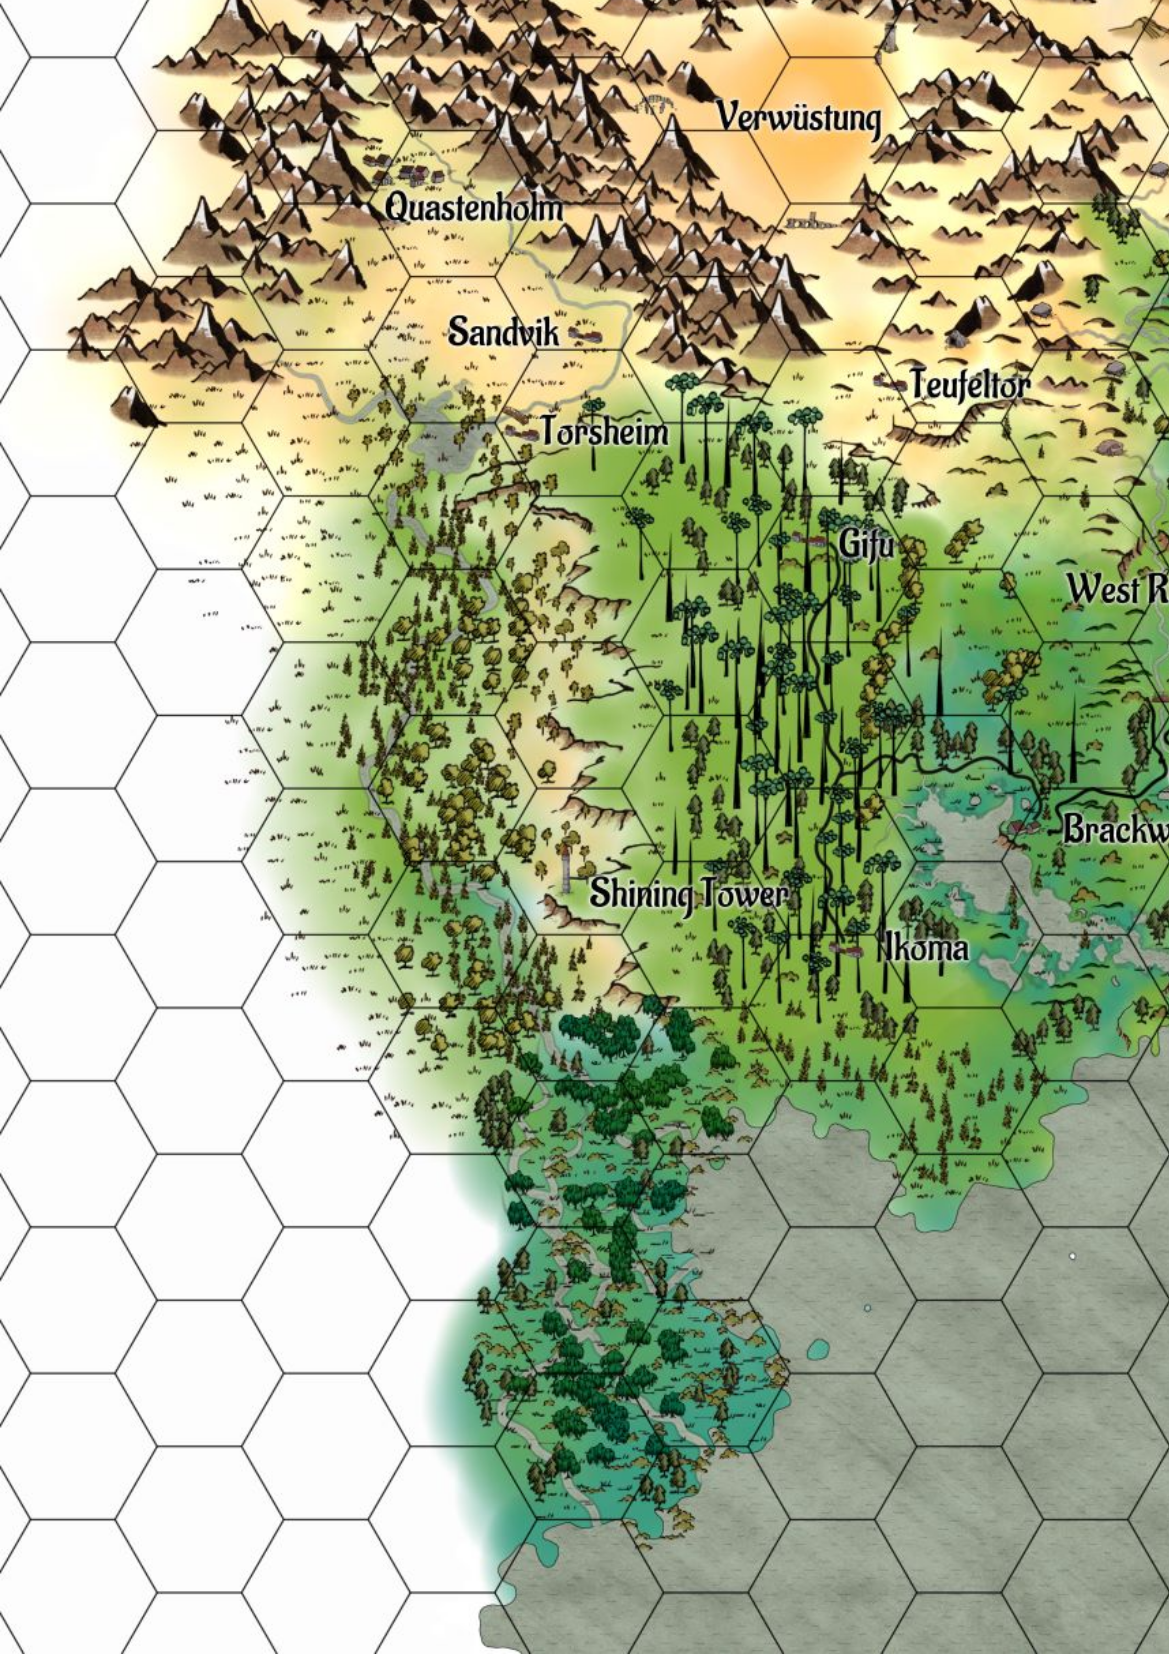
\includepdf{Backcover.pdf}
\end{document}
